\documentclass[11pt]{article}
\usepackage[utf8]{inputenc}

%%%%%% LAYOUT %%%%%%%
\usepackage[margin=1in]{geometry} %Ask before changing or deleting this line.

%%%%%% USEFUL PACKAGES %%%%%%

\usepackage{amsmath,amssymb,amsfonts,amsthm}
\usepackage{enumitem}
\usepackage{multicol}

%%%%%% MAKING DIAGRAMS %%%%%%

\usepackage{asymptote} %Very powerful 
\usepackage{tikz} %Good for drawing graphs
\usepackage{graphicx} %Allows you to include external image files
\usepackage{ytableau} %Good for making Young tableaux
\usepackage{youngtab} %Good for making simple Young tableaux

%%%%%% USEFUL COMMANDS %%%%%%

%Feel free to add your own shorthands here.
\newcommand{\bN}{\mathbb{N}}
\newcommand{\bZ}{\mathbb{Z}}
\newcommand{\bR}{\mathbb{R}}
\newcommand{\bC}{\mathbb{C}}
\newcommand{\bQ}{\mathbb{Q}}
\newcommand{\bF}{\mathbb{F}}
\newcommand{\bP}{\mathbb{P}}
\newcommand{\To}{\Rightarrow}           %% entre funtores
\newcommand{\ov}{\overline}        %% short for  \overline
\newcommand{\cM}{\mathcal{M}}           %% multiplicadores
\newcommand{\set}[1]{\{\,#1\,\}}    %% set notation
\newcommand{\obonj}[1]{\left\rbrack#1\right\lbrack}
\newcommand*{\Cdot}{{\raisebox{-0.25ex}{\scalebox{1.5}{$\cdot$}}}}      %% cdot más grande
\DeclareMathOperator{\PGL}{PGL} %%% grupo proyectivo lineal
\newcommand{\twobyone}[2]{\begin{pmatrix} %% 2 x 1 matrix
    #1 \\ #2 \end{pmatrix}}
 \newcommand{\twobytwo}[4]{\begin{pmatrix} %% 2 x 2 matrix
    #1 & #2 \\ #3 & #4 \end{pmatrix}}
\newcommand{\less}{\setminus}           %% set difference

\newtheorem{theorem}{Theorem}
\newtheorem{prop}[theorem]{Proposition}
\newtheorem{corollary}[theorem]{Corollary}
\newtheorem{lemma}[theorem]{Lemma}
\newtheorem{conjecture}[theorem]{Conjecture}
\newtheorem{Th}{Theorem}               %%% Theorem 1.1.1
\newtheorem{Tmon}{Teoremón}
\newtheorem{Prop}{Proposition}         %%% Proposition 1.1.2
\newtheorem{Lem}{Lemma}                 %%% Lemma 3
\newtheorem{Cor}{Corollary}            %%% Corollary 4

\theoremstyle{definition}

\newtheorem{definition}[theorem]{Definition}
\newtheorem{remark}[theorem]{Remark}
\newtheorem{example}[theorem]{Example}
\newtheorem{Def}{Definition}           %%% Definition 5
\newtheorem{Ex}{Example}               %%% Example 6
\newtheorem{Ej}{Exercise}             %%% Exercise 7

\theoremstyle{remark}
\newtheorem{Rmk}[Th]{Remark}      %%%Remark 1.1.9
\newtheorem*{nonum-Rmk}{Remark}         %%% No number Fact
\newtheorem*{Notn}{Notation}        %% Notaciones
\newtheorem*{Warn}{Warning}       %% Warnings

\numberwithin{theorem}{section}



%%%%% TITLE, AUTHOR %%%%%

\title{Moduli Spaces of Stable Curves with Marked Points: Examples and Connections to Trees.}
\author{Ignacio Rojas}
\date{Spring, 2023}


\begin{document}

\maketitle
\begin{abstract}
    This work explores the concept of moduli spaces of stable curves with marked points, which are sets of parameters describing families of objects. These spaces can be used to solve problems in enumerative geometry, such as determining the number of curves passing through a given number of points. The common principle underlying these solutions is the association of the objects with a moduli space, which provides a different perspective on the problem. We illustrate this connection with examples.
    \end{abstract}
    
    \begin{flushleft}
    \small
    \emph{Keywords}:
    moduli space, curves enumerative geometry, parametrization.
    
    \emph{MSC classes}:  Primary \texttt{14D22}; Secondary \texttt{05C05, 14H10}.
    \end{flushleft}
\section{Introduction}

Let us begin with a simple question:
\begin{center}\begin{minipage}{0.9\textwidth}\centering\em
    Which are the quadratic curves which pass through $4$ points in $\bR^2$ and no three of them are collinear?
\end{minipage}\end{center}
This question might be a bit tough to tackle right now, but let us simplify. How about if the points are $(1,1),(1,-1),(-1,-1)$ and $(-1,1)$? At once the following idea should pop-in in our heads: \emph{a circle}! The circle which passes through these points is described by the equation $x^2+y^2=2$ as seen in Figure \ref{fig1}.
\begin{figure}[h!]
    \centering
    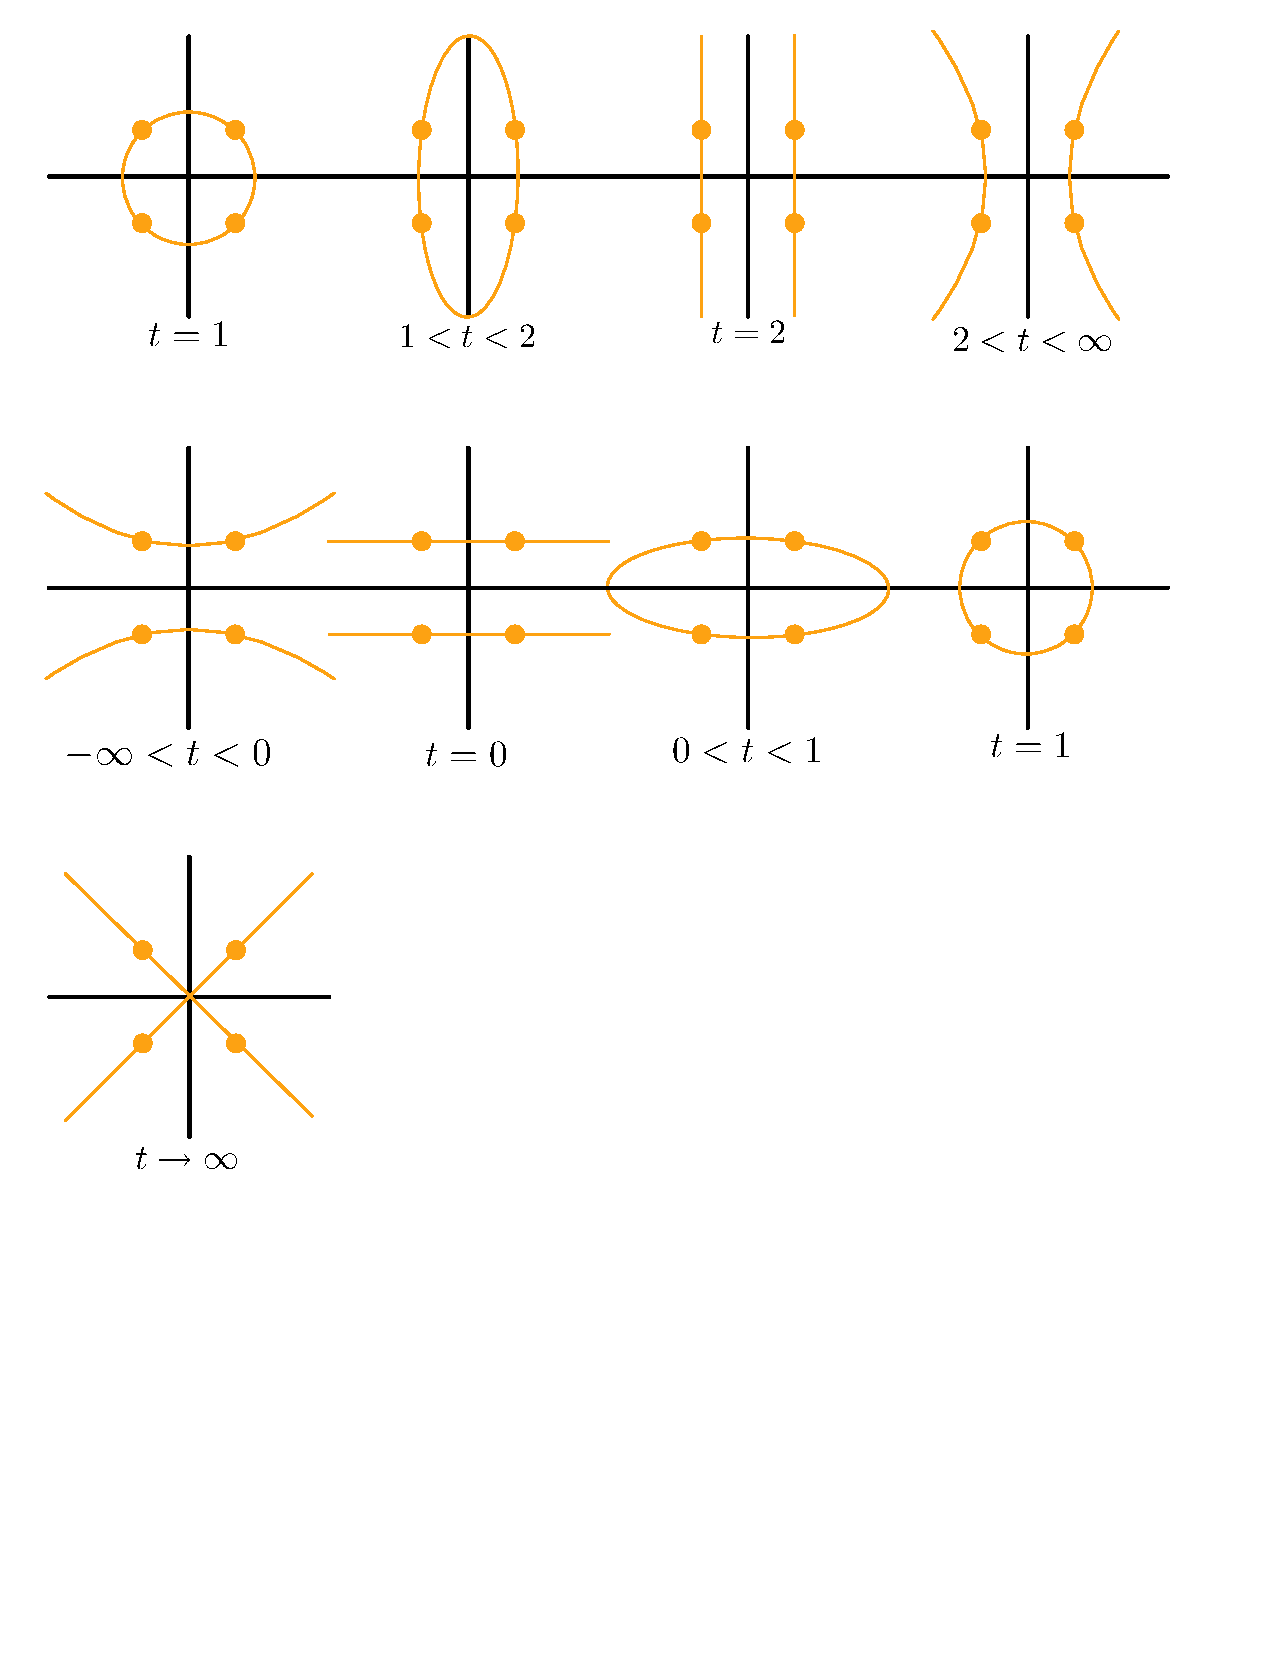
\includegraphics[width=0.3\textwidth, trim= 0.8cm 22.9cm 16cm 0.6cm,clip]{fig1.pdf}
    \label{fig1}
    \caption{One of the quadratic curves passing through our points: $x^2+y^2=2$.}
\end{figure}
Ideally we would like to stretch and shrink the circle in order to make it an ellipse. We know ellipses have equations of the form $x^2/a^2+y^2/b^2=1$, but to begin from our circle equation we will instead add coefficients to the equation 
$$Ax^2+By^2=2.$$
These coefficients are determined by the points on the curve, we may derive the relation by plugging in a point into the equation:
$$A(1)^2+B(1)^2=2\To B=2-A\To tx^2+(2-t)y^2=2$$
where we take $t=A$ to get the last equation.
We annotate the curves we obtain given different values of $t$:
\vspace{-0.5em}
\begin{itemize}
    \begin{multicols}{2}
        \itemsep=-0.4em
    \item $(t=1)$: A circle.
    \item $(1<t<2)$: An ellipse.
    \item $(t=2)$: The pair of lines $x^2=1$.
    \item $(t>2)$: A hyperbola.
    \end{multicols}
\end{itemize}
However we are left with one curve which passes through the points in question. To find it we will assume $t$ is non-zero. From our parametric equation we obtain 
$$tx^2+(2-t)y^2=2\To x^2+o(t)+y^2=\frac{2}{t}\xrightarrow[t\to\infty]{}x^2=y^2$$
which is the pair of lines $y=\pm x$. Observe that this behavior is independent of the sign of the infinity we are going to. 
\begin{figure}[h!]
    \centering
    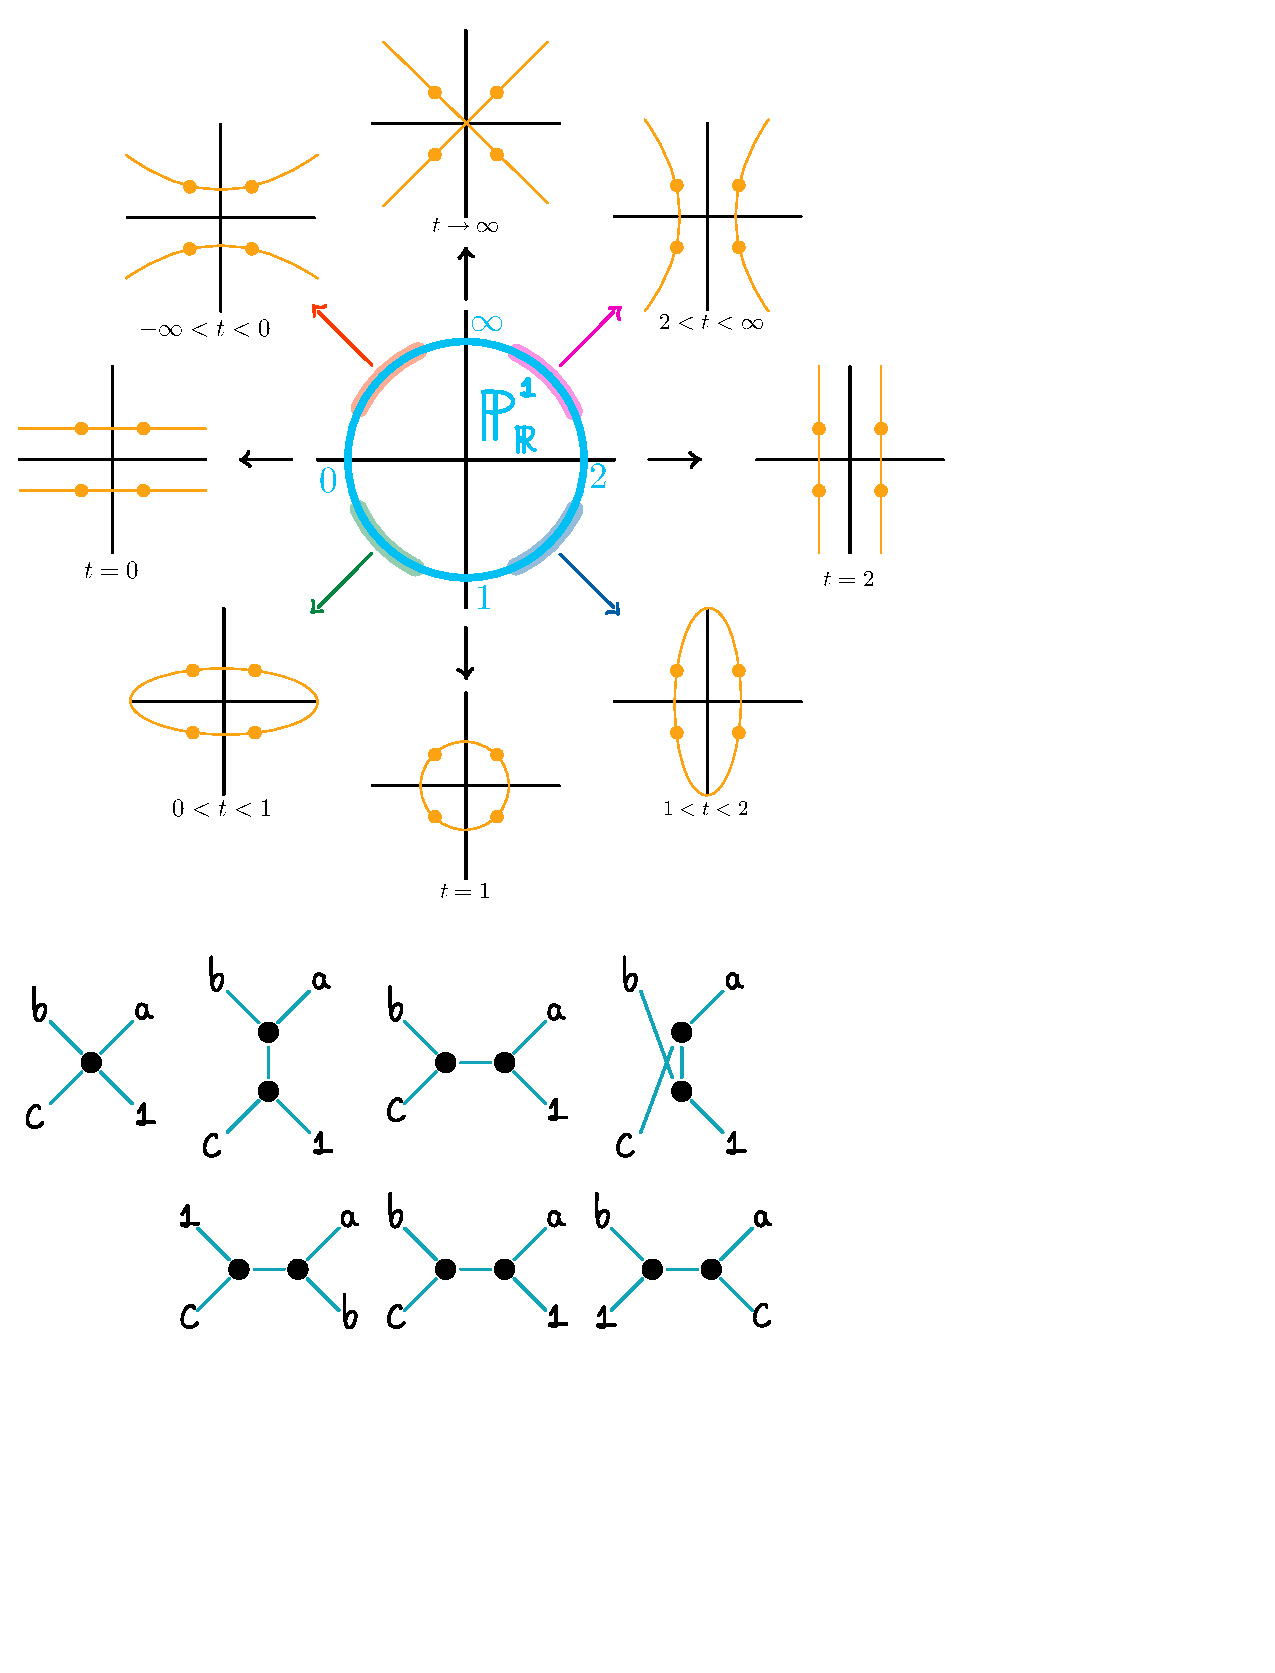
\includegraphics[width=0.8\textwidth, trim= 0.25cm 13.1cm 5.25cm 0.5cm,clip]{fig2.pdf}
    \label{fig2}
    \caption{The projective real line as the moduli space $\ov\cM_{0,4}$.}
\end{figure}
In essence what we have seen is that all the quadratic curves passing through our set of points can be parametrized by $\bR\cup\set{\infty}$. Formally:
\begin{Prop}
The moduli space $\ov{\cM}_{0,4}$ can be identified with $\bP^1_\bR$.
\end{Prop}
Intuitively the moduli space is a set of parameters. When the points vary \emph{continuously}, the objects they parametrize deform \emph{continuously} as well. What we have done here is not a proof of the previous proposition but it may serve as evidence that it is true.\par 
To study this space and other spaces which may arise in this fashion, we may ask a question like \emph{how many such curves can we find?} In order to do this, we will address this problem by connecting it with graphs. 

\section{Connection with trees}

As a first approach we could consider an incidence graph where our vertices are the marked points and they are connected if they are in the same component of our curve. However that might produce undesirable results as it could lead to disconnected graphs.

\begin{Def}
For a point in $\ov{\cM}_{0,X}$ (which represents a curve), we define the \underline{dual tree} to that curve as:
\begin{itemize}
    \item $V=X\cup I$ where $I$ is the set of irreducible components in our curve. The set $X$ attaches \textbf{labels} to our vertices while the curves are unlabeled.
    \item Vertices in $X$ are not connected between themselves, but $u\in X$ is adjacent to $v\in I$ if $u$ lies in the irreducible component associated to $v$.\par 
    For $u,v\in I$, $uv$ is an edge if the components meet at a nodal singularity.
\end{itemize}
\end{Def}

Even though we have defined the dual tree to be a tree, it may not be totally clear why this is the case: \textbf{buajaja figure \ref{fig2} \ref{fig1}}
\begin{center}\begin{minipage}{0.9\textwidth}\centering\em
    Why should this process generate a tree? Why not a disconnected graph or a cycle?
\end{minipage}\end{center}
This follows from the definition because we are talking about \emph{genus $0$} curves. When we admit holes, what we are allowing in the graph is cycles.

\begin{Ex}
Let us consider the case of $\ov\cM_{0,4}$, our labeled vertices will be 
$$a=(1,1),\quad b=(-1,1),\quad c=(-1,-1),\quad 1=(-1,-1).$$
We have different types of trees:
\begin{enumerate}
    \itemsep=-0.4em
    \item For ellipses and circles, the vertices are ${a,b,c,1}$ or ${\cdot}$, and the edges are of the form $x\cdot$ for $x\in X$. This gives us a $K_{1,4}$ graph.
    \item Hyperbolas have a unique component. In the projective plane, the components are connected at the point corresponding to the \emph{slope of the asymptotes} at infinity, so the dual trees of the hyperbolas are also $K_{1,4}$ graphs.
    \item For $t=0$, there are two unlabeled vertices. $a$ and $b$ are connected to one vertex, while $c$ and $1$ are connected to the other. At infinity, there is a nodal singularity at the point corresponding to the slope of the lines, which means they connect.\par 
    A similar analysis can be done for $t=2$ and $t\to\infty$, and the resulting graph is two copies of $P_3$ connected by their middle vertices.
\end{enumerate}
The corresponding trees are shown in the following figure: 
\begin{figure}[h!]
    \centering
    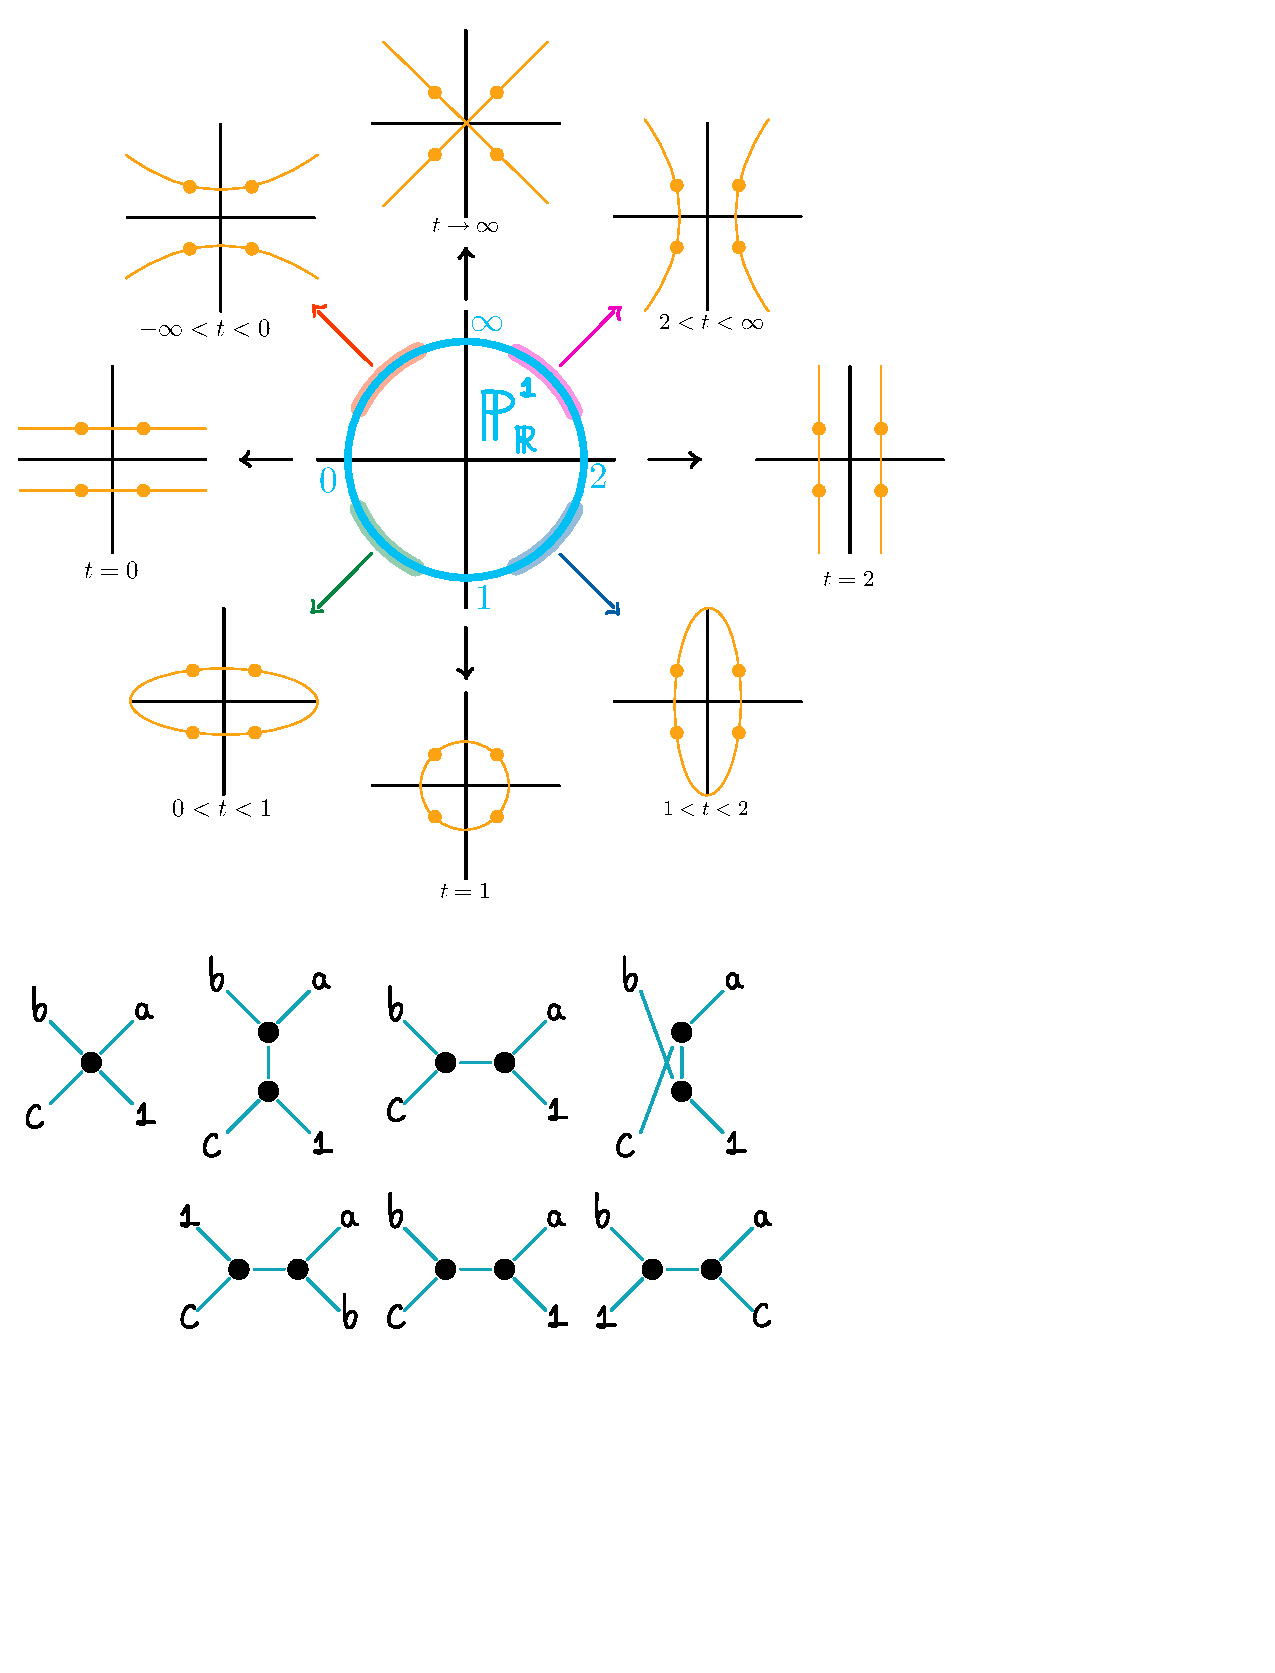
\includegraphics[width=0.8\textwidth, trim= 0.4cm 8.3cm 9cm 16cm,clip]{fig2.pdf}
    \label{fig3}
    \caption{Trees associated to: $(1)$ circles, ellipses and hyperbolas; $(2)$ the curve $y^2=1$; $(3)$ the curve $x^2=1$; and $(4)$ the curve $x^2=y^2$.}
\end{figure}
\end{Ex}

\begin{Rmk}
Look at the degrees of our vertices, there are no vertices of degree 2. If we remove the labels, all the trees besides $(1)$ are isomorphic.\par
Also notice that when talking about the ellipses and the circle, we did not assign a particular value of $t$ to each of the curves. We just said \emph{an ellipse} or also \emph{an hyperbola}, which means that the whole family of those curves is associated to the particular tree we obtained.
\end{Rmk}

\begin{Def}
For a tree $T$ we have that:
\begin{enumerate}
    \itemsep=-0.4em
    \item $T$ is \underline{trivalent} if all vertices of $T$ have degree $1$ or $3$ and at least one vertex has degree $3$.
    \item $T$ is \underline{at least trivalent} if no vertex of $T$ has degree $2$ and at least one vertex has degree at least $3$.
\end{enumerate}
\end{Def}

\begin{Rmk}
In our graphs, observe that the trees associated to \emph{families} of curves like ellipses and hyperbolas, correspond to \emph{at least trivalent} trees.\par 
While for the particular cases $t=0$, $t=2$ and $t\to\infty$ we get exactly \emph{trivalent} trees. \emph{This is no coincidence!} The fact that at least trivalent trees correspond to a large number of curves and that the trivalent ones only to a select few.
\end{Rmk}

\begin{Def}
    The \underline{boundary stratum} corresponding to a tree $T$ is the set of curves whose dual tree is $T$. 
\end{Def}

\begin{Ex}
In our example, the boundary stratum of $K_{1,4}$ is $$\obonj{-\infty,0}\cup\obonj{0,2}\cup\obonj{2,\infty}$$
where we identify $\infty$ with $-\infty$.\par 
The remaining points $\set{0},\set{2}$ and $\set{\infty}$ are \emph{zero-dimensional} and these are the boundary points which correspond to the trivalent trees.
\end{Ex} 

The observation that the boundary points correspond to the trivalent trees is key, because knowing this allows us to simplify the problem of counting the boundary points to counting \emph{certain} trivalent trees. In general this result is true:

\begin{Prop}
    The boundary points of $\ov\cM_{0,X}$ correspond to trivalent trees whose leaf set is labeled with $X$. If $X=\set{a,b,c,1,2,\dots,n}$, then the number of boundary points of $\ov\cM_{0,X}$ is $(2n+1)!!$. 
\end{Prop}

To count the number of leaf-labeled trivalent trees $L_n$ on $n+3$ leaves, we begin with the following small values:
\begin{itemize}
    \item When $n=0$, there is only one tree, $K_{1,3}$, with a unique labeling of the leaves. So $L_0=1$, which coincides with $(2(0)+1)!!=1$.
    \item When $n=1$, we have two copies of $P_3$ joined by their middle vertices. There are $4!$ ways to label the four leaves without constraints. Accounting for symmetries, we have $L_1=4!/2^3=3$, as pictured in the Figure \ref{fig3} above.
    \item For the next case we are supposed to find $15$ trees. Counting by hand or considering symmetries is not the way to go. We've got to be more creative than that. A question arises:
    \begin{center}\begin{minipage}{0.9\textwidth}\centering\em
        Is there a way to obtain the next trees from the old trees?
    \end{minipage}\end{center}
    In essence, we wish to add a new leaf to our graph. Intuitive ways in which we could proceed are:
    \begin{itemize}
        \item Adding the leaf to a leaf vertex. But this actually doesn't work. We add one leaf but we lose one and even worse, now one vertex \textbf{has degree 2}. This means our tree is \textbf{no longer trivalent}.
        \item Adding the leaf to a non-leaf vertex. Indeed we now have a new leaf, but the vertex we added to now has \textbf{degree 4}. So our tree is \textbf{no longer trivalent}.
    \end{itemize}
    Apparently our original ideas won't work. So with a boost of creativity we will instead pop the leaf \emph{out of an edge}:\par
    \begin{figure}[h!]
        \centering
        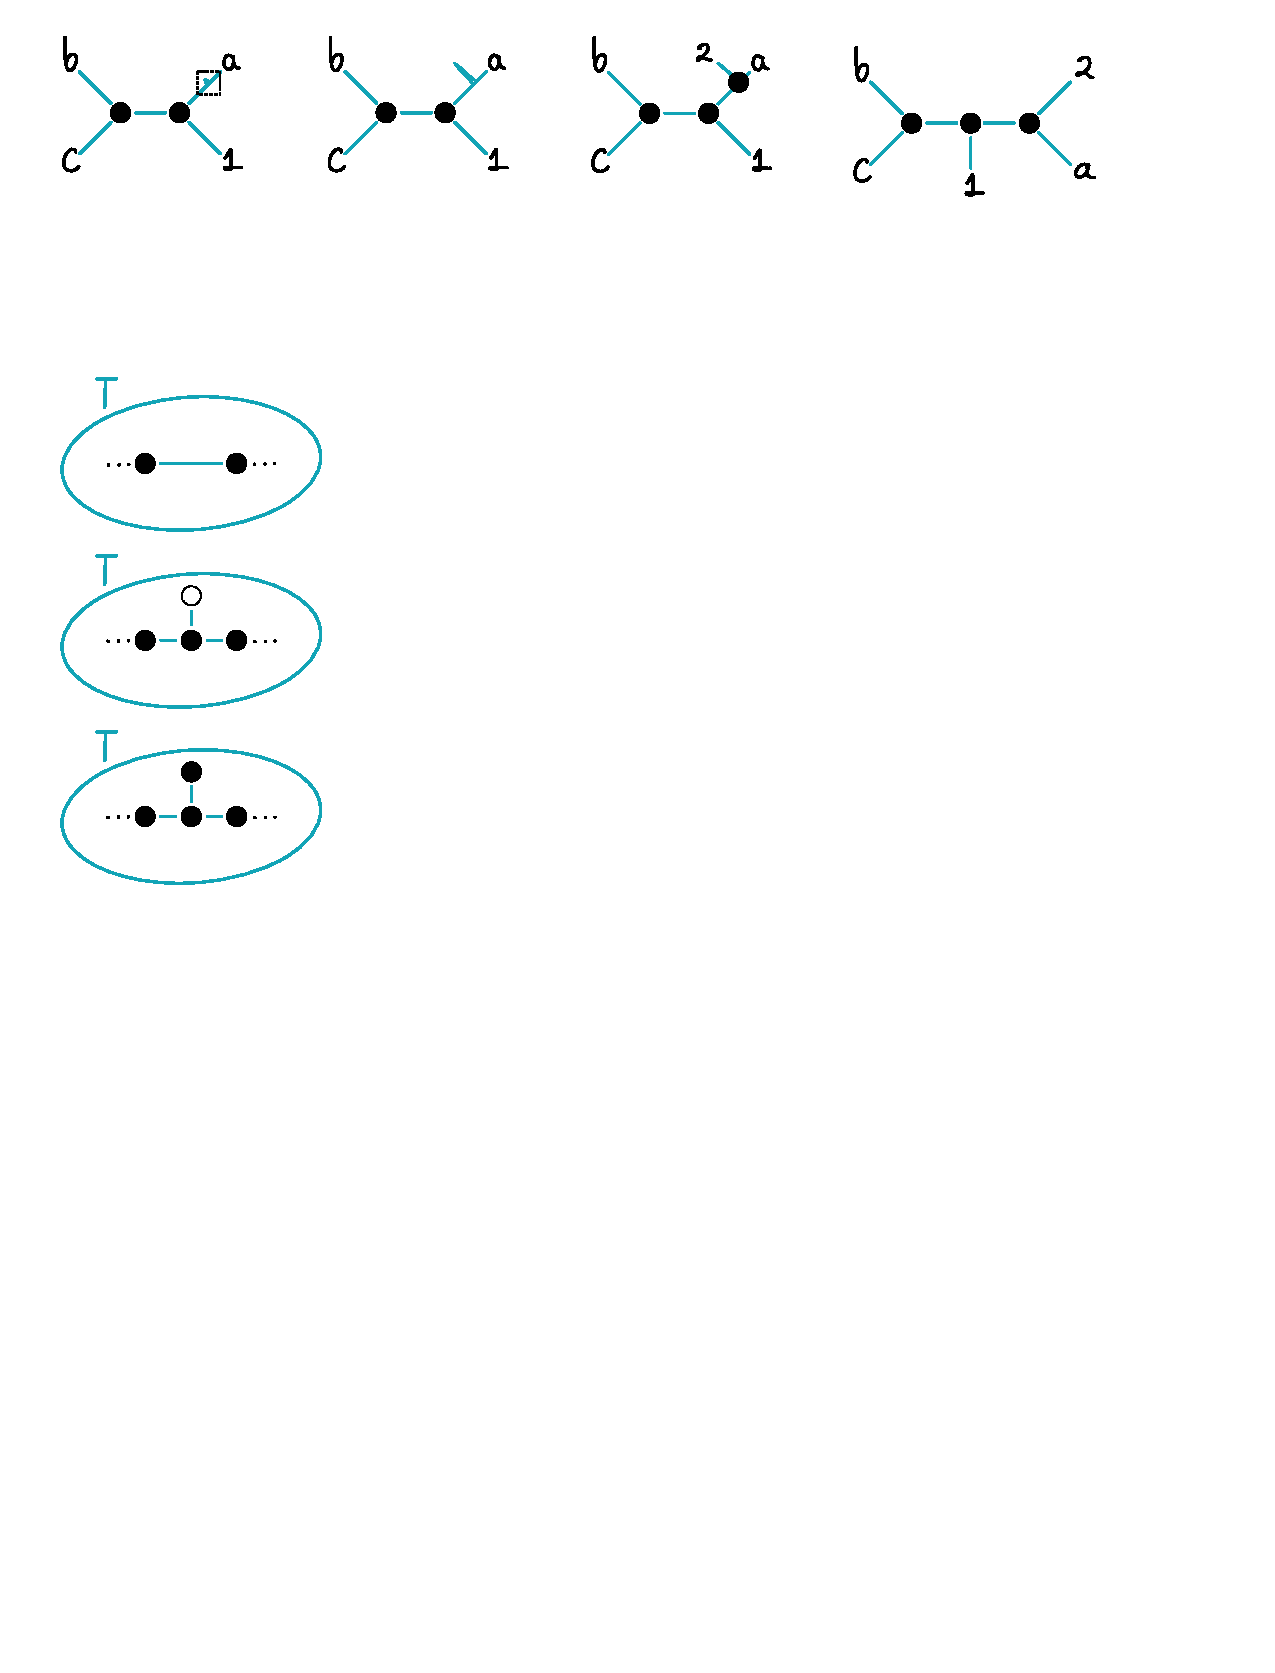
\includegraphics[width=0.8\textwidth, trim= 1cm 25cm 3.05cm 0.65cm,clip]{fig3.pdf}%LDRU
        \label{fig4}
        \caption{\emph{Popping} a leaf out of an edge to form a new trivalent tree.}
    \end{figure}
    Note that adding a leaf to an edge creates a new vertex with degree $3$ and adds a new leaf to the tree. There is no constraint on the number of vertices in a trivalent tree, so we can add as many new leaves as we want.\par 
    Back to our three trees, each one has 5 edges which means there are 5 possible ways to add a labeled leaf. This gives us a total of 15 ways to form a 5-leaved labeled trivalent tree from the previous ones. Thus, $L_2=15$, which is equal to $(2\Cdot2+1)!!=1\Cdot3\Cdot5$.
    \item For $n=3$, we count leaf-labeled trivalent trees with $6$ leaves. Each of our $15$ previous trees has $7$ edges to which we can adjoin a new labeled leaf. For each of the trees, these are different possibilities. So in total we have $7\Cdot L_2=105$ new trees. 
\end{itemize}

We formalize this strategy using a couple of lemmas:

\begin{Lem}
The number of edges $E_n$ on a trivalent tree with $n+3$ leaves satisfies the recursion:
$$E_n=E_{n-1}+2,\quad E_0=3$$
which means that $E_n=2n+3$.
\end{Lem}

\begin{proof}
    We will proceed using induction. The base cases have been discussed earlier, so now we will use an $(n-1)+3=n+2$ leaved trivalent tree as a starting point.\par 
To add a new leaf while preserving the trivalent property, we add a new vertex to an existing edge and attach the leaf to that vertex. This process creates two new edges: 
\begin{itemize}
    \item One edge which was split in two by the addition of the new vertex in the middle.
    \item Another one created by attaching the leaf to the new vertex.
\end{itemize}
  This means that the number of edges increased by two and the degree of the new vertex is $3$, so $E_n=E_{n-1}+2$ as desired. The recursion can be solved using the initial condition to obtain $E_n=(2n+3)$ for all $n$.
\end{proof}

\begin{Lem}
The number of leaf-labeled trivalent trees with $n+3$ leaves, $L_n$, satisfies the recursion 
$$L_{n}=E_{n-1}L_{n-1},\quad L_0=1.$$ 
\end{Lem}

\begin{proof}
    The base cases have been proven in the previous discussion. So for an $(n+2)$-leaved tree, we have ${a,b,c,1,2,\dots,n-1}$ as the labels of our leaves.\par 
    Adding the leaf labeled $n$ can be done in $E_{n-1}$ ways because we may attach it to any of the existing edges. Each of these new trees has a unique set of labels, and there are $L_{n-1}$ such trees. Therefore, there are $E_{n-1}L_{n-1}$ new leaf-labeled trivalent trees.\par 
    Solving the recursion we have $L_n=(2n+1)L_{n-1}$ which means that 
    $$L_n=(2n+1)(2n-1)(2n-3)\dots=(2n+1)!!.$$
\end{proof}

With these results in hand the proposition is immediately true. The fact the boundary points correspond to the trivalent trees is a consequence of the fact that automorphisms of $\bP^1$ are determined by $3$ points.

\section{But what really is $\ov{\cM}_{0,n}$?}

Up to now we've referred to $\ov{\cM}_{0,4}$, so let us concretely explain what that space is by answering a couple of questions:
\begin{enumerate}
    \itemsep=-0.4em
    \item On its own, without the closure, what is $\cM_{0,4}$?
    \item What is being added with the closure, and what topology are we working with?
\end{enumerate}

To address these questions we refer to \cite{RenzoNotes} and \cite{cavalieri2021projective}. 
\iffalse
\begin{Def}
    The \underline{moduli space} $\cM_{0,n}$ parametrizes genus $0$ curves with $n$ marked points.
\end{Def}

It is a lucky coincidence that the only genus $0$ curve is \textbf{ASK MARK/MARIA} so this definition can be restated with this in mind. 
\fi
\begin{Def}
    The \underline{moduli space} $\cM_{0,n}$ parametrizes ordered $n$-tuples of distinct points in $\bP^1$ up to \emph{projective equivalence}. Two arrays of points $(p_1,\dots,p_n),\ (q_1,\dots,q_n)$ are equivalent when 
    $$\exists T\in\PGL_2\left[(q_1,\dots,q_n)=(Tp_1,\dots,Tp_n)\right].$$
    In our case $\cM_{0,4}$ can be seen to be the set of \emph{equivalence classes} of arrays $(p_1,\dots,p_4)$ with $p_i\in\bP^1$. 
\end{Def}

\begin{Rmk}
    Drawing an analogy with matrices, where the row-reduced echelon form serves as a canonical representative of the equivalence class of row-equivalent matrices, we seek a similar notion of canonical representation for the moduli space $\cM_{0,4}$.
\end{Rmk}

\begin{Prop}
    Any projective transformation $T\in\PGL_2$ is determined by where it maps $0,1$ and $\infty$. 
\end{Prop}

The proof of this fact is a basic computation in linear algebra.

\begin{Rmk}
    Before starting the proof, we point out a caveat. The projective transformation that we will find here maps $0,1$ and $\infty$ to $3$ points $p_1,p_2,p_3$.\par 
    The inverse of this transformation is the one that we use to find a representative of the equivalence class. Because it maps our points $p_1,p_2,p_3$ to $0,1,\infty$. 
\end{Rmk}

\begin{proof}
    Assigning coordinates we have 
    $$0=[0:1],\quad 1=[1:1],\quad \infty=[1:0].$$
    Now suppose $T=\twobytwo{t_{11}}{t_{12}}{t_{21}}{t_{22}}$ is a projective transformation and $p,q,r$ are points in $\bP^1$ such that
    $$
    \left\lbrace
    \begin{aligned}
        &T[1:0]=p=[p_1:p_2]\\
        &T[0:1]=q=[q_1:q_2]\\
        &T[1:1]=r=[r_1:r_2]
    \end{aligned}
    \right.
    $$
    From the first two equations we have that 
    $$\twobyone{t_{11}}{t_{21}}=m_1\twobyone{p_1}{p_2},\quad\text{and}\quad\twobyone{t_{12}}{t_{22}}=m_2\twobyone{q_1}{q_2}\quad\text{for some}\quad m_1,m_2\neq 0$$
    which means that the columns of $T$ are proportional to $p$ and $q$ and to determine $T$ we are only required to determine $m_1$ and $m_2$. Replacing these entries into the matrix and considering the last equation we have 
    $$\twobytwo{m_1p_1}{m_2q_1}{m_1p_2}{m_2q_2}\twobyone{1}{1}=m_3\twobyone{r_1}{r_2}\To \left\lbrace
    \begin{aligned}
        &m_1p_1+m_2q_1=m_3r_1,\\
        &m_1p_2+m_2q_2=m_3r_2,
    \end{aligned}
    \right.\To \twobytwo{p_1}{q_1}{p_2}{q_2}\twobyone{m_1}{m_2}=\twobyone{m_3r_1}{m_3r_2}.$$
    The last matrix's columns are linearly independent because they are the image of two l.i. vectors under a linear transformation. This means that we may recover $(m_1,m_2)$ by inverting that matrix:
    $$\twobyone{m_1}{m_2}=m_3\twobytwo{p_1}{q_1}{p_2}{q_2}^{-1}\twobyone{r_1}{r_2}.$$
    This information determines $T$ up to a scalar multiple $m_3$ which means that projectively, we have determined $T$.
\end{proof}

With the proposition in hand we may map the first $3$ points of our array to the special points $0,1,\infty$, and let the last one map to an arbitrary but fixed $t$:
$$(Tp_1,\dots,Tp_4)=(0,1,\infty,t),\quad t\in\bP^1.$$
At the level of equivalence classes this means:
$$[(\bP^1,(p_1,\dots,p_4))]=[(\bP^1,(0,1,\infty,t))]$$
and so every equivalence class of points is determined by a unique $t\in\bP^1$.

\begin{Rmk}
Recall that in the definition of the moduli space, we stated that the points $(p_1,\dots,p_4)$ should be \textbf{distinct}! So this means that $t$ is not in the whole of $\bP^1$, $t$ can't be $0,1$ nor $\infty$. 
\end{Rmk}

The previous discussion proves the following result.

\begin{Prop}
    The moduli space $\cM_{0,4}$ is isomorphic to $\bP^1\less\set{0,1,\infty}$.
\end{Prop}

Our intuition points to the fact that the closure of $\cM_{0,4}$ will include the values of $\bP^1$ that we have excluded. The compactification process we describe is the Deligne-Mumford compactification, even though there are other possible ways to compact this space.

\begin{Def}
    The space $\ov{\cM}_{0,n}$ parametrizes pg 30modulaiespeises
\end{Def}



%%%%%%%%%%%% Contents end %%%%%%%%%%%%%%%%
\nocite{*}
\bibliographystyle{plain}
\bibliography{bibiProyCombi2.bib}

\end{document}